\documentclass{beamer}

\usetheme{Frankfurt}
%\usetheme{Warsaw}

%\usepackage{ragged2e}
\usepackage{graphicx}

\usepackage[justification=centering]{caption}

\usepackage{rotating}

\usepackage{amsmath}
\usepackage{amssymb}
\usepackage{yquant}
\useyquantlanguage{groups}
\usetikzlibrary{fit, quotes}
\usetikzlibrary{snakes,arrows,shapes}

\usepackage{graphicx}

\usepackage{float}
\usepackage{hyperref}
\usepackage{physics}
\def\be#1\ee{\begin{equation}#1\end{equation}}

\usepackage[utf8]{inputenc}

\usepackage{color}
%\usepackage[dvipsnames]{xcolor}

\renewcommand{\mark}			{{\bf Oznaczenie: \\}}
\renewcommand{\det}[1]			{det \left( #1 \right)}
\renewcommand{\ker}[1]			{ker \left( #1 \right)}
\renewcommand{\limits}[1]		{\left. #1 \right|}
\renewcommand{\d}				{\delta}
\newcommand{\tg}[2]			{tg^{#1}\parenthesis{#2}}
\newcommand{\ctg}[2]			{ctg^{#1}\parenthesis{#2}}

\newcommand{\im}[1]				{Im \left( #1 \right)}
\newcommand{\task}[1]			{{\bf Zadanie #1.}\\}
\newcommand{\observation} 		{{\bf Obserwacja:}\\}
\newcommand{\property}[1] 		{{\bf Wlasnosci } #1 :\\ }
\newcommand{\theoremName}[1]	{{\bf Twierdzenie (#1):}}
\newcommand{\conclusion}		{{\bf Wniosek:}}
\newcommand{\remark}			{{\bf Uwaga:\\}}
\newcommand{\question}			{{\bf Pytanie:\\}}
\newcommand{\mb}[1] 			{\mathbb{#1}}
\newcommand{\mc}[1]				{\mathcal{#1}}
\newcommand{\ilim}[1]			{lim_{#1 \to \infty}}
\newcommand{\zlim}[1]			{lim_{#1 \to 0}}
\newcommand{\pdiv}[2]			{\frac{\partial #1}{\partial #2}}
\newcommand{\dive}[2]			{\frac{d #1}{d #2}}
\newcommand{\pdivpt}[3]			{\left. \frac{\partial #1}{\partial #2} \right|_{#3}}
\newcommand{\ndimfunc}[1]		{\left\{ 
	\begin{array}{ll}
		#1
	\end{array}
	\right.}
\newcommand{\colvec}[1]			{\left[
	\begin{array}{c}
		#1
	\end{array}
	\right]}
\newcommand{\rowvec}[1]			{\left[
	#1
	\right]}
\newcommand{\cmatrix}[2]		{\left[
	\begin{array}{#1}
		#2
	\end{array}
	\right]}
\newcommand{\parenthesis}[1]	{\left( #1 \right)}
\newcommand{\brackets}[1]		{\left\{ #1 \right\}}
\newcommand{\linSys}[1]			{
	\left\{ 
	\begin{array}{l}
		#1
	\end{array} 
	\right.
}
\newcommand{\e}					{\epsilon}
\renewcommand{\d}				{\delta}
\renewcommand{\a}				{\alpha}
\renewcommand{\b}				{\beta}
\newcommand{\lin}[1]			{\left< #1 \right>}
\newcommand{\sprod}[2]			{\left< \left. #1 \right| #2 \right> }
\newcommand{\x}					{\times}
\newcommand{\subs}[1]			{
	\left/ \left/
	\begin{array}{l}
		#1
	\end{array}
	\right/ \right/
}
\newcommand{\ver}[1]			{\hat{e}_{#1}}
\newcommand{\p}[1]				{\partial_{#1}}
\newcommand{\tdiv}				{\frac{d}{dt}}

\newcommand\blfootnote[1]{%
  \begingroup
  \renewcommand\thefootnote{}\footnote{#1}%
  \addtocounter{footnote}{-1}%
  \endgroup
}

\usepackage{physics}

\newcommand{\gcm}{{\color{OliveGreen} \checkmark}}
\newcommand{\rx}{{\color{red} $\times$}}

% Define custom colors
\definecolor{codeblue}{rgb}{0.25,0.5,0.75}
\definecolor{backgray}{rgb}{0.95,0.95,0.95}

\usepackage{listings}
% Python code style
\lstdefinestyle{pythonstyle}{
	language=Python,                 % Use Python language
	backgroundcolor=\color{backgray}, % Set background color
	commentstyle=\color{OliveGreen},       % Comments in green
	keywordstyle=\color{blue},        % Keywords in blue
	stringstyle=\color{codeblue},     % Strings in light blue
	basicstyle=\ttfamily\footnotesize,% Basic font style
	frame=single,                     % Frame the code
	breaklines=true,                  % Allow breaking lines
	numbers=left,                     % Line numbers on the left
	numberstyle=\tiny\color{gray},    % Line number style
	tabsize=4,                        % Set tab size to 4 spaces
	showstringspaces=false,            % Do not show spaces in strings
	morekeywords = {QMLModel, ModelFinder}
}
\lstset{style=pythonstyle}





\usepackage{amsmath,epsfig,mathrsfs,graphicx,amssymb,color,float}
\usepackage[T1]{fontenc}
\usepackage{t1enc}
\usepackage{hyperref}
\usepackage{array}
\usepackage{booktabs}
\usepackage{ulem}

\newcommand{\h}[1]{\hat{ #1}}
\newcommand{\f}[2]{\frac {#1}{#2}}
\def\e{\boldsymbol e}
\def\p{\partial}
\newcommand{\g}[1]{{\boldsymbol #1}}
\def\rmd{\mathrm d}
\def\rmi{\mathrm i}
\def\rme{\mathrm e}
\def\be#1\ee{\begin{equation}#1\end{equation}}
\newcommand{\ba}{\begin{eqnarray} }
	\newcommand{\ea}{\end{eqnarray} }
\def\cor#1{{\color{red}#1}}
\def\kor#1{{\color{blue}#1}}



\usepackage{amsmath,epsfig,mathrsfs,graphicx,amssymb,color,float}
\usepackage[T1]{fontenc}
\usepackage{t1enc}
\usepackage{hyperref}
\usepackage{array}
\usepackage{booktabs}
\usepackage{ulem}


\def\e{\boldsymbol e}
\def\p{\partial}
\def\rmd{\mathrm d}
\def\rmi{\mathrm i}
\def\rme{\mathrm e}
\def\be#1\ee{\begin{equation}#1\end{equation}}
\def\cor#1{{\color{red}#1}}
\def\kor#1{{\color{blue}#1}}



%PAKIETY
%\usepackage[cp1250]{inputenc}   % pozwala wprowadza��„�¢Â€Â¡ polskie znaki bezpo�„¹�¢Â€Âºrednio z klawiatury
\usepackage{amsmath}            % AMS-LaTeX (AMS-Math)
\usepackage{amsfonts}           % ekstra fonty matematyczne
\usepackage{amssymb}            % ekstra symbole matematyczne
%\usepackage{a4wide}             % szersza kolumna tekstu ni�„¹�„½ domy�„¹�¢Â€Âºlnie
\usepackage{enumerate,graphicx}
%\usepackage{multicol}
\usepackage{array}
\usepackage{booktabs}
\usepackage{bbm}
\usepackage{physics}

%PAKIETY
%\usepackage{polski}             % spolszczenie LaTeXa
%\usepackage[utf8]{inputenc}   % pozwala wprowadza�¦ polskie znaki bezpoœrednio z klawiatury
\usepackage{amsmath}            % AMS-LaTeX (AMS-Math)
\usepackage{amsfonts}           % ekstra fonty matematyczne
\usepackage{amssymb}            % ekstra symbole matematyczne
% szersza kolumna tekstu ni¿ domyœlnie
\usepackage{enumerate,graphicx}
\usepackage{array}
\usepackage{booktabs}
\usepackage{yquant}
\usetikzlibrary{fit, quotes}
\usetikzlibrary{snakes,arrows,shapes}
\useyquantlanguage{groups}
\usepackage{physics}
\usepackage{todonotes}
\newtheorem{thm}{Theorem}





\setbeamersize{text margin left=5mm,text margin right=5mm} 

\def\arraystretch{1.5} % Rozciąga wysokość tablicy

\setbeamertemplate{navigation symbols}{} % remove navigation symbols
\setbeamertemplate{footline}[frame number]

\title[\tiny LGI-based benchmark]{Leggett-Garg Inequality-based Quantum Computers Quality Benchmark}

\author[Tomek Rybotycki, Adam Bednorz]{\textbf{Tomek Rybotycki}, \textbf{Adam Bednorz}}
\institute[SRI PAS]{
	Systems Research Institute, Polish Academy of Sciences\\
	Nicolaus Copernicus Astronomical Center, Polish Academy of Sciences\\
	Center of Excellence in Artificial Intelligence, AGH University of Cracow\\
	Faculty of Physics, University of Warsaw
}

\date{
	IQM Research Awards 2026 Finals\\
	19 VIII 2026, Online
}
%\logo{
%	
\includegraphics[height=1cm]{figs/logos/ibs_pan_CMYK.pdf}%
% 	
\includegraphics[height=1cm]{figs/logos/camk.pdf}
% 	
\includegraphics[height=1cm]{figs/logos/ceai-logo-icon.png}
% 	
\includegraphics[height=1cm]{figs/logos/EN_zwykly_okragly.png}
% 	% TODO: ADD FUW LOGO
% }


\begin{document}
	
	%\justifying
	
	\frame{\titlepage}
	
	\begin{frame}{Motivation}
		
		\begin{block}{European Quantum Strategy}

			Our research are aligned with the European Quantum Strategy.			

			\begin{itemize}

				\item The need for independent benchmarking tools.
				
				\item Testing under-explored properties of quantum devices.
				
				\item Unexplained error sources found in previous research.

			\end{itemize}
			
		\end{block}
	
		\begin{block}{Constellation-topology devices}
			
			With the advent of Constellation-topology devices, more attention
			should be given to devices with central resonators.
			
			\begin{itemize}

				\item Software for devices with central resonator (e.g. Qubit Selector)
				
				\item Benchmarks that promote high inter-qubit connectivity.
				
				\item Dedicated implementation of weak measurements using
				pulse-level access.
				
			\end{itemize}
			
		\end{block}	
	
	\end{frame}


	\begin{frame}{Executive summary}
		
		\vspace{-0.3cm}
		
		\begin{block}{Primary research}
			We propose Leggett-Garg inequality-based benchmark that is:
			\begin{itemize}

				\item Highly scalable (different topologies, parallelization),
				
				\item Versatile: application to benchmarking partially entangling gates and pulse control,
				
				\item Extendable (pulse-controlled weak coupling, more qubits...),
				
				\item Robust to noise.
				
			\end{itemize}
		\end{block} 
	
		\vspace{-0.2cm}
	
		\begin{block}{Technical results}
			We present repository with the code we produced. Therein:
			\begin{itemize}

				\item Implementation of benchmark circuits, experimental
				pipelines and analysis scripts.
				
				\item Qubit Selector for Star-shaped topology devices. Expandable to Constellation-topology devices.
				
				\item Simulators based on the historical calibration data.
				
			\end{itemize}
		\end{block}
	
	
	\end{frame}
	
	
	\begin{frame}{Projective vs weak measurement}

		\vspace{-0.4cm}
		
		\begin{columns}
			
			\begin{column}{0.5\textwidth}
				\begin{block}{Projective (strong) measurement}
				
					\begin{itemize}
						\item Direct
						\item Accurate (in theory)
						\item Disturbing (decoherence)
					\end{itemize}
					\begin{center}
						\begin{figure}[height=2cm]
							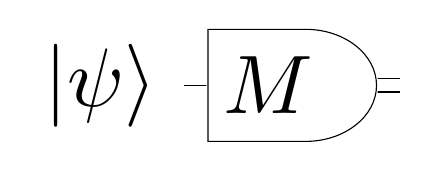
\begin{tikzpicture}[scale=3]
								\begin{yquant*}
									qubit {} q[1];
									init  {$\ket \psi$} q[0];
									dmeter {$M$} q[0];
								\end{yquant*}
							\end{tikzpicture}
						\end{figure}
					\end{center}
				\end{block}
			\end{column}
			
			
			\begin{column}{0.5\textwidth}
				\begin{block}{Weak measurement}
					\begin{itemize}
						\item Indirect (weak coupling)
						\item Inaccurate (deliberately)
						\item Small decoherence
					\end{itemize}
					\begin{center}
						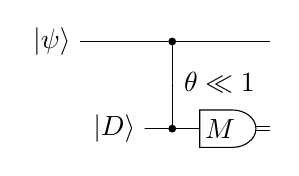
\begin{tikzpicture}[scale=1]
							\begin{yquant*}
								qubit {} q[3];
								discard q[1,2];
								init  {$\ket \psi$} q[0];
								init {$\ket D$} q[2];
								[shape=yquant-circle, radius=0mm]
								box {} q[1] |  q[0],q[2];
								hspace {-3mm} q[1];
								text {$\theta\ll 1$} q[1];
								dmeter {$M$} q[2];
							\end{yquant*}
						\end{tikzpicture}
					\end{center}	
				\end{block}
			\end{column}
		
		
		\end{columns}

	
		\begin{alertblock}{No free lunch}
			\begin{itemize}
				\item Information gain $>\theta$
				\item Decoherence $>\theta^2$
			\end{itemize}
		\end{alertblock}
	
	
		\begin{alertblock}{The catch: Measurement strength $\theta$ calibration}
			$a_{raw}=\theta a_{physical}$
		\end{alertblock}
	
	
	\end{frame}


	\begin{frame}{Application: Leggett-Garg inequality violation}

		\begin{block}{Leggett-Garg (LG) Inequality}
		$$
		\langle a \rangle + \langle b \rangle - \langle ab \rangle \leq 1, \:|a|\leq 1,|b|\leq 1
		$$
		\end{block}

	
		\begin{columns}
			\begin{column}{0.5\textwidth}
				\begin{block}{LG-based benchmark inequality}
					$$
						Q = \frac{\braket{a}{c}\braket{b}{c}}{\braket{ab}{c}} \leq 1,
					$$
					where $\langle ab|c\rangle=\langle abc\rangle/p(c=1)$.
					\begin{itemize}
						\item measurement strength-agnostic
						\item postselection $c=0,1$,
						\item  $A\equiv B$ (identical, independent)
					\end{itemize}
	
				
				\end{block}
			\end{column}
		
			\begin{column}{0.5\textwidth}
				\begin{center}
					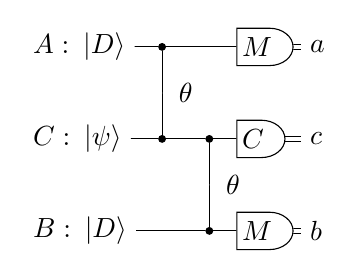
\begin{tikzpicture}[scale=1]
						\begin{yquant*}
							qubit {} q[5];
							discard q[0,1,2,3,4];
							% q[1];
							%init  q[0];
							align q[0],q[2],q[4];
							init {$C:\:\ket \psi$} q[2];
							init {$A:\:\ket D$} q[0];
							init {$B:\:\ket D$} q[4];
							%
							[shape=yquant-circle, radius=0mm]
							box {} q[1] |  q[0],q[2];
							hspace {-3mm} q[1];
							text {$\theta$} q[1];
							%
							[shape=yquant-circle, radius=0mm]
							box {} q[3] |  q[4],q[2];
							hspace {-3mm} q[3];
							text {$\theta$} q[3];
							align q[0],q[2],q[4];
							dmeter {$M$} q[0];
							output {$a$} q[0];
							dmeter {$C$} q[2];
							output {$c$} q[2];
							dmeter {$M$}  q[4];
							output {$b$} q[4];
						\end{yquant*}
					\end{tikzpicture}
				\end{center}
			\end{column}
	
		\end{columns}
	
		\begin{block}{Detectors identity and independence ($A \equiv B$)}
			
			Partially verifiable by $D = 0$, where $D := \langle a \rangle \langle bc \rangle - \langle b \rangle \langle ac \rangle $.
			
		\end{block}
	
	
	\end{frame}



	\begin{frame}{A test with strength dependence on $\lambda=\sin\theta$}
		\vspace{-1cm}
		\begin{columns}
			
			\begin{column}{0.4\textwidth}
				\begin{block}{Setup}
					$$A = B = Z = \ketbra{0} - \ketbra{1}$$
					$$C = \ketbra{\psi_-} $$
					$$\ket{\psi} = \ket{\psi_+}$$
					$$
					\ket{\psi_\pm} = \cos \frac{\psi}{2}\ket{1} \pm \sin \frac{\psi}{2}\ket{0}
					$$
				\end{block}
			\end{column}
			
			
			\begin{column}{0.6\textwidth}
				\begin{figure} 
					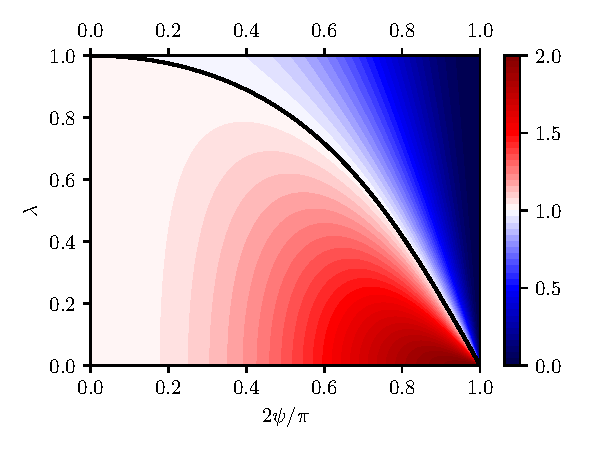
\includegraphics[scale=.7]{figs/lgapar.pdf}
				\end{figure} 
			\end{column}
		
		
		\end{columns}
		
		\begin{block}{Benchmark scores}
			\begin{itemize}
				\item Simple: $B_S = (Q-1)/\sigma = n_\sigma$
				\item Normalized (one-tailed confidence): $B_N = \frac{1}{2} \mathrm{erf}\left( \frac{n_\sigma}{\sqrt{2}} \right)  $
			\end{itemize}
		\end{block}
		
	\end{frame}
	
	
		
	\begin{frame}{Weak coupling implementation}
		\vspace{-0.2cm}
		
		\begin{columns}
			
			\begin{column}{0.6\textwidth}
		
				\begin{block}{Outline}
					\begin{itemize}
						\item Two qubit gate $U\sim I$
						\item Basis: $\ket{00}, \ket{01}, \ket{10}, \ket{11}$
					\end{itemize}	
				\end{block}
			
				\begin{block}{Weak coupling with IQM-native gates}
					
					We use two $CZ$ gates sandwiching $Y_\theta$ gate.
					
					\begin{figure}	
						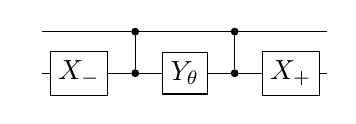
\begin{tikzpicture}[scale=1]
							\begin{yquant*}
							qubit {} q[2];
								init {} q[0];
								init {} q[1];
								box {$X_-$} q[1];
								zz (q[0],q[1]);
								box {$Y_\theta$} q[1];
								zz (q[0],q[1]);
								box {$X_+$} q[1];
								\end{yquant*}
							\end{tikzpicture}
					\end{figure}
				\end{block}

		
	
			\end{column}
		
			\begin{column}{0.3\textwidth}
				\begin{block}{Notation}
					$ X = \ketbra{0}{1} + \ketbra{1}{0}$
					$ Y = i \ketbra{1}{0} - i \ketbra{0}{1}$
					$ V_\theta = \exp(-i\theta V)$
					$ V_\pm = V_{\pm\pi/2}$		
				\end{block}
			\end{column}
			
		
		\end{columns}
	
		\begin{block}{Alternative: Fractional gates}
			
			Weak coupling implementation is native on IBM / IonQ devices with
			the fractional RZZ gate.
			
			$$
				RZZ(\theta) = \mathrm{diag}(1, e^{i\theta}, e^{i\theta}, 1)
			$$
			
		\end{block}
		
	\end{frame}




	\begin{frame}{Experiments: Detectors independence ($\theta = 0.1$)}

		\begin{columns}
			
			\begin{column}{0.5\textwidth}
				
				\begin{block}{IQM Sirius}
					\begin{figure}
						
						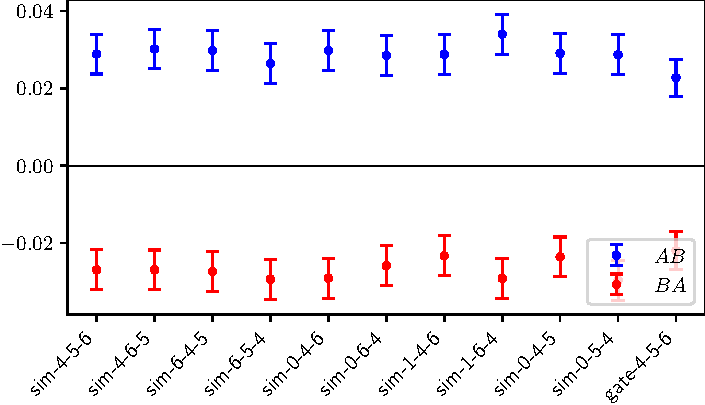
\includegraphics[width=\textwidth]{figs/detectors_iqm_sirius.pdf}
						
						\begin{itemize}
							\item CAB qubits specified
							\item $10^6$ shots per qubits set
							\item $D$ within > 5 $\sigma$ from 0
							\item Simulator close to real device
						\end{itemize}
						
					\end{figure}
				\end{block}
				
			\end{column}
		
			\begin{column}{0.5\textwidth}
				
				\begin{block}{IQM Emerald}
					\begin{figure}
						
						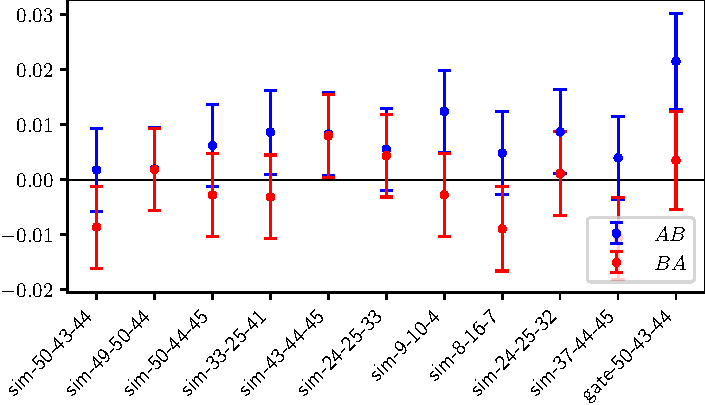
\includegraphics[width=\textwidth]{figs/detectors_iqm_emerald.pdf}
						
						\begin{itemize}
							\item CAB qubits specified
							\item $10^6$ shots per qubits set
							\item $D$ within < 1 $\sigma$ from 0
							\item Simulation far from real device
						\end{itemize}
						
					\end{figure}
				\end{block}
				
			\end{column}
			
		\end{columns}

	\end{frame}



	\begin{frame}{Experiments: Benchmark score ($\theta = 0.1$)}
		
		\vspace{-0.25cm}
		
		\begin{columns}
			
			\begin{column}{0.48\textwidth}
				
				\begin{block}{IQM Sirius}
					\begin{figure}
						
						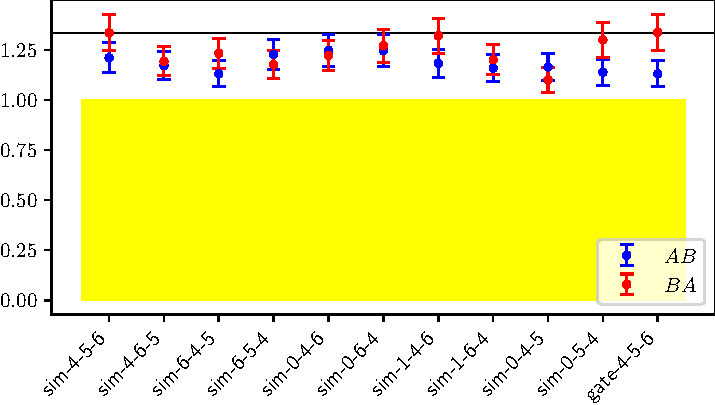
\includegraphics[width=\textwidth]{figs/benchmark_iqm_sirius.pdf}
												
					\end{figure}
				
					Benchmark values (on device):
					\begin{itemize}

						\item $B_S^{AB} = 1.9954, \; B_S^{BA} = 3.7494$
						
						\item $B_N^{AB} = 0.9770, \; B_N^{BA} = 0.9999$
						
					\end{itemize}
				
				\end{block}
				
			\end{column}
			
			\begin{column}{0.48\textwidth}
				
				\begin{block}{IQM Emerald}
					\begin{figure}
						
						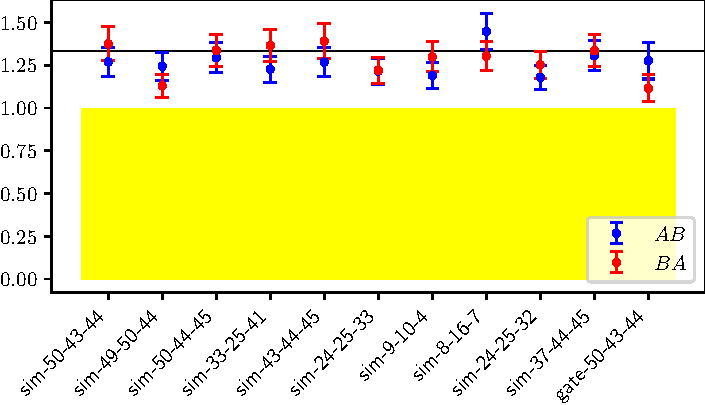
\includegraphics[width=\textwidth]{figs/benchmark_iqm_emerald.pdf}
											
					\end{figure}
				
					Benchmark values (on device):
					\begin{itemize}
						
						\item $B_S^{AB} = 2.5935, \; B_S^{BA} = 1.4625$
						
						\item $B_N^{AB} = 0.9253, \; B_N^{BA} = 0.9282$
						
					\end{itemize}
				
				\end{block}
				
			\end{column}
			
		\end{columns}
	
		\begin{alertblock}{Shots number}
			The results could be improved with better statistics.
		\end{alertblock}
		
	\end{frame}


	
	\begin{frame}{Experiments: Different providers ($\theta = 0.1$)}

	\vspace{-0.4cm}
	
	\begin{columns}
		\begin{column}{0.48\textwidth}
			\begin{block}{IBM Kingston (RZZ, $2 \cdot 10^7$ shots)}
				\begin{center}
					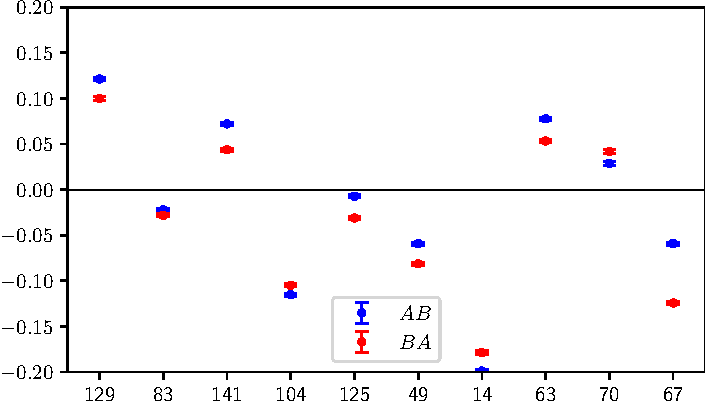
\includegraphics[scale=.4]{figs/dzzki.pdf}
					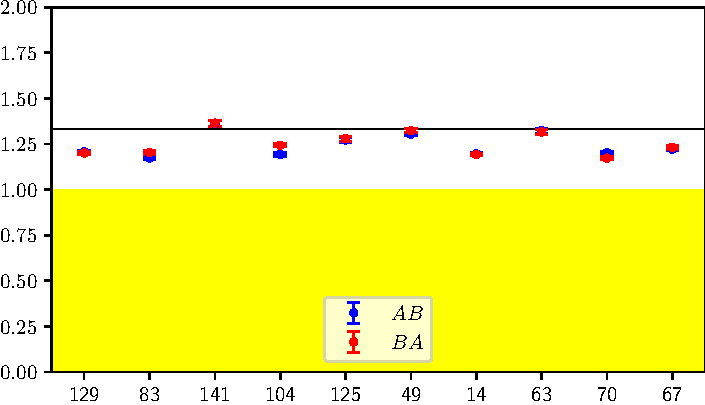
\includegraphics[scale=.4]{figs/lgazzki.pdf}		
				\end{center}
			\end{block}
		\end{column}
		\begin{column}{0.48\textwidth}		
			\begin{block}{IBM Kingston (CZ, $2 \cdot 10^7$ shots)}
				\begin{center}
					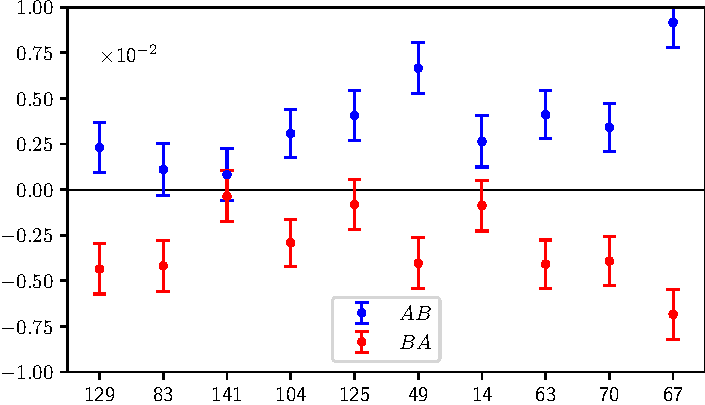
\includegraphics[scale=.4]{figs/dczki.pdf}
					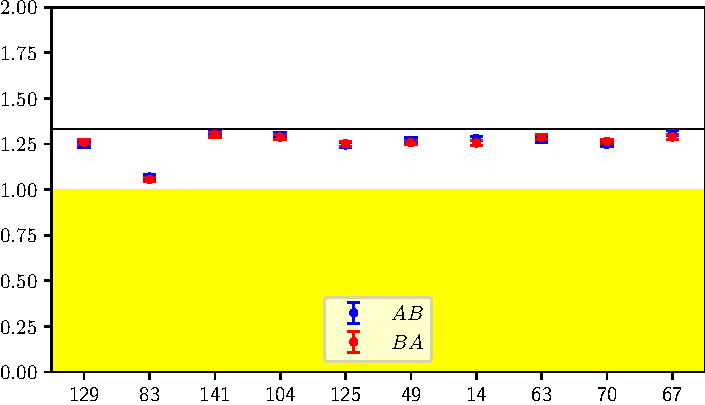
\includegraphics[scale=.4]{figs/lgaczki.pdf}	
				\end{center}
			\end{block}
		\end{column}
		\end{columns}
		\begin{block}{IonQ Forte}
				IonQ Forte 1: $1.272\pm 0.035$ ($A\to B$),
	$1.289 \pm 0.035$ ($B\to A$)
		\end{block}
	\end{frame}




	\begin{frame}{Failed Experiment: IQM Pulla}
		
		\begin{columns}
			
			\begin{column}{0.47\textwidth}
				
				\begin{itemize}

					\item IQM Sirius
					
					\item \# shots = $10^6$
					
					\item qubits: [4, 5, 6] (best set)
					
					\item Measurement pulse amplitude halved for all qubits
										
				\end{itemize}
		
				\begin{alertblock}{Conclusions}
					\begin{itemize}
						
						\item Naive pulse modification lead to poor results
						
						\item In some cases, benchmark inequality may still
						be violated
						
					\end{itemize}
				\end{alertblock}
				
			\end{column}
		
			\begin{column}{0.47\textwidth}
				
				\begin{block}{Detectors validation}
					
					\begin{itemize}

						\item $D_{AB} = -0.000871 \pm 0.005872$
						
						\item $D_{BA} = -0.000068 \pm 0.005807$

					\end{itemize}
					
				\end{block} 
				
				\begin{block}{Benchmark Scores}
					
					\begin{itemize}

						\item $Q_{AB} = 0.8012 \pm 0.3660$
												
						\item $Q_{BA} = 1.8411 \pm 1.9617$
						
						\item $B_S^{AB} = -0.543063$
					
						\item $B_N^{AB} = 0.293543$
					
						\item $B_S^{BA} = 0.428756$
					
						\item $B_N^{BA} = 0.665950$
						
					\end{itemize}
				\end{block}
				
			\end{column}
			
		\end{columns}

	\end{frame}


	\begin{frame}{Impact and directions}
		
		\vspace{-0.3cm}
		
		\begin{block}{Impact}
			\begin{itemize}
				
				\item New benchmarking protocol for different properties of the device
				
				\item Benchmarking partially entangling gates and pulse control
				
				\item Robustness to noise -- no error correction needed
				
				\item Minimal disturbance: $\theta=0.1 \to $ disturbance $1/400$
				
				\item Device-agnostic (highly scalable)
				
			\end{itemize}
		\end{block}
	
		\vspace{-0.2cm}
		
		\begin{block}{Research directions}

			\begin{itemize}

				\item Test benchmark limits with sufficient statistics ($\sigma\sim 1/\theta^2\sqrt{N}$)
				
				\item Weak coupling implementation using pulse-level control
				e.g. creating continuous families of entangling gates ($CZ\to \mathrm{diag}(1,1,1,e^{\pm i\theta})$)
				
				\item Avoid postselection (full noninvasiveness)
				
				\item Scaling up the test. Extend qubits sets on star topology
				devices. Benchmark score extension for whole device.
				
				\item Investigate the reason of $D$ increase in $RZZ$ protocol version.
				
			\end{itemize}
		\end{block}
		
	\end{frame}


	\begin{frame}{Thank you for your attention!}

		\vspace{-0.3cm}

		\begin{block}{Special thanks to:}
			\begin{itemize}
				\item Our long-standing collaborators/supporters: 
				\begin{itemize}
					\item Wolfgang Belzig
					\item Jakub Tworzyd{\l}o
					\item Josep Batle
				\end{itemize}
							
				\item Device providers: IQM, IBM, IonQ
				
				\item  Pozna{\'n} Supercomputing and Networking Center -- Polish access hub
			\end{itemize}
				
		\end{block}
	
		\vspace{-0.3cm}
	
		\begin{columns}
			
			\begin{column}{0.3\textwidth}
				\begin{center} 
					\begin{block}{Repository}
						\begin{figure} 
							
\includegraphics{figs/IQM_repo_QR.png}
						\end{figure}
					\end{block}
				\end{center}
			\end{column}
				
			\vspace{-0.3cm}	
			
			\begin{column}{0.60\textwidth}
				\begin{center}
					
					\begin{block}{Our LG manuscripts}
						\begin{figure}
							
\includegraphics{figs/LG_QR.png}
							
\includegraphics{figs/LGA_QR.png}
						\end{figure}
					\end{block}
				\end{center}
			\end{column}
	
			
		\end{columns}
	
	\end{frame}

	


\end{document}
